\section{Empirical Evaluation}
\label{sec:lso:experiments}
This section aims to empirically answer three main questions:
\begin{enumerate}
    \item How does weighted training affect the latent space of \glspl{dgm}? (\S\ref{subsec:expt-weighting})
    \item How do the parameters of weighted retraining influence optimisation? (\S\ref{subsec:expt-wr})
    \item Does weighted retraining compare favourably to existing methods? (\S\ref{subsec:expt-baselines})
\end{enumerate}
To answer these questions, we perform experiments using three optimisation tasks 
chosen to represent three different data and model types.
The tasks are described in \S\ref{sec:lso:expt-tasks}.
Because there is no obvious single metric to evaluate sample-efficient optimisation,
we choose to plot the $K$th best novel evaluated point as a function of the number of objective function evaluations,
which we denote as the \emph{Top$K$} score.
All plots show the average performance and standard deviation across runs with 5 different random seeds unless otherwise stated.
This evaluation method is common practice in Bayesian optimisation \citep{shahriari2015taking}.
It contrasts with previous works which typically report only final scores,
and take the maximum across seeds rather than the average
\citep{gomez2018,kusner_grammar_2017,dai_syntax-directed_2018,jin_junction_2019}.

All experimental data and code to reproduce the experiments can be found at 
\codelink{}.

\subsection{Tasks}
\label{sec:lso:expt-tasks}

\subsubsection{2D Shape Area Maximisation Toy Task}
As a simple toy task that can be easily visualized in 2D,
we optimise for the shape with the largest total area in the space of $64\times64$ binary images
(i.e.\@ the largest number of pixels with value 1).

\paragraph{Data} A dataset of $\approx$10,000 squares of different sizes and positions
on a $64\times64$ background, with a maximum area of 400
(see \cref{fig:shape-samples} for examples).
\paragraph{Model} A convolutional \gls{vae} with $\Z=\mathbb{R}^2$,
as a standard neural network architecture for image modelling.
It was implemented using PyTorch \citep{paszke2019pytorch} and PyTorch Lightning \citep{falcon2019pytorch}.
\paragraph{Latent optimiser} We enumerate a grid in latent space over $[-3,+3]^2$,
to emulate a perfect optimiser for illustration purposes (this is only feasible since $\Z$ is low-dimensional).

\begin{figure}[ht]
    \centering
    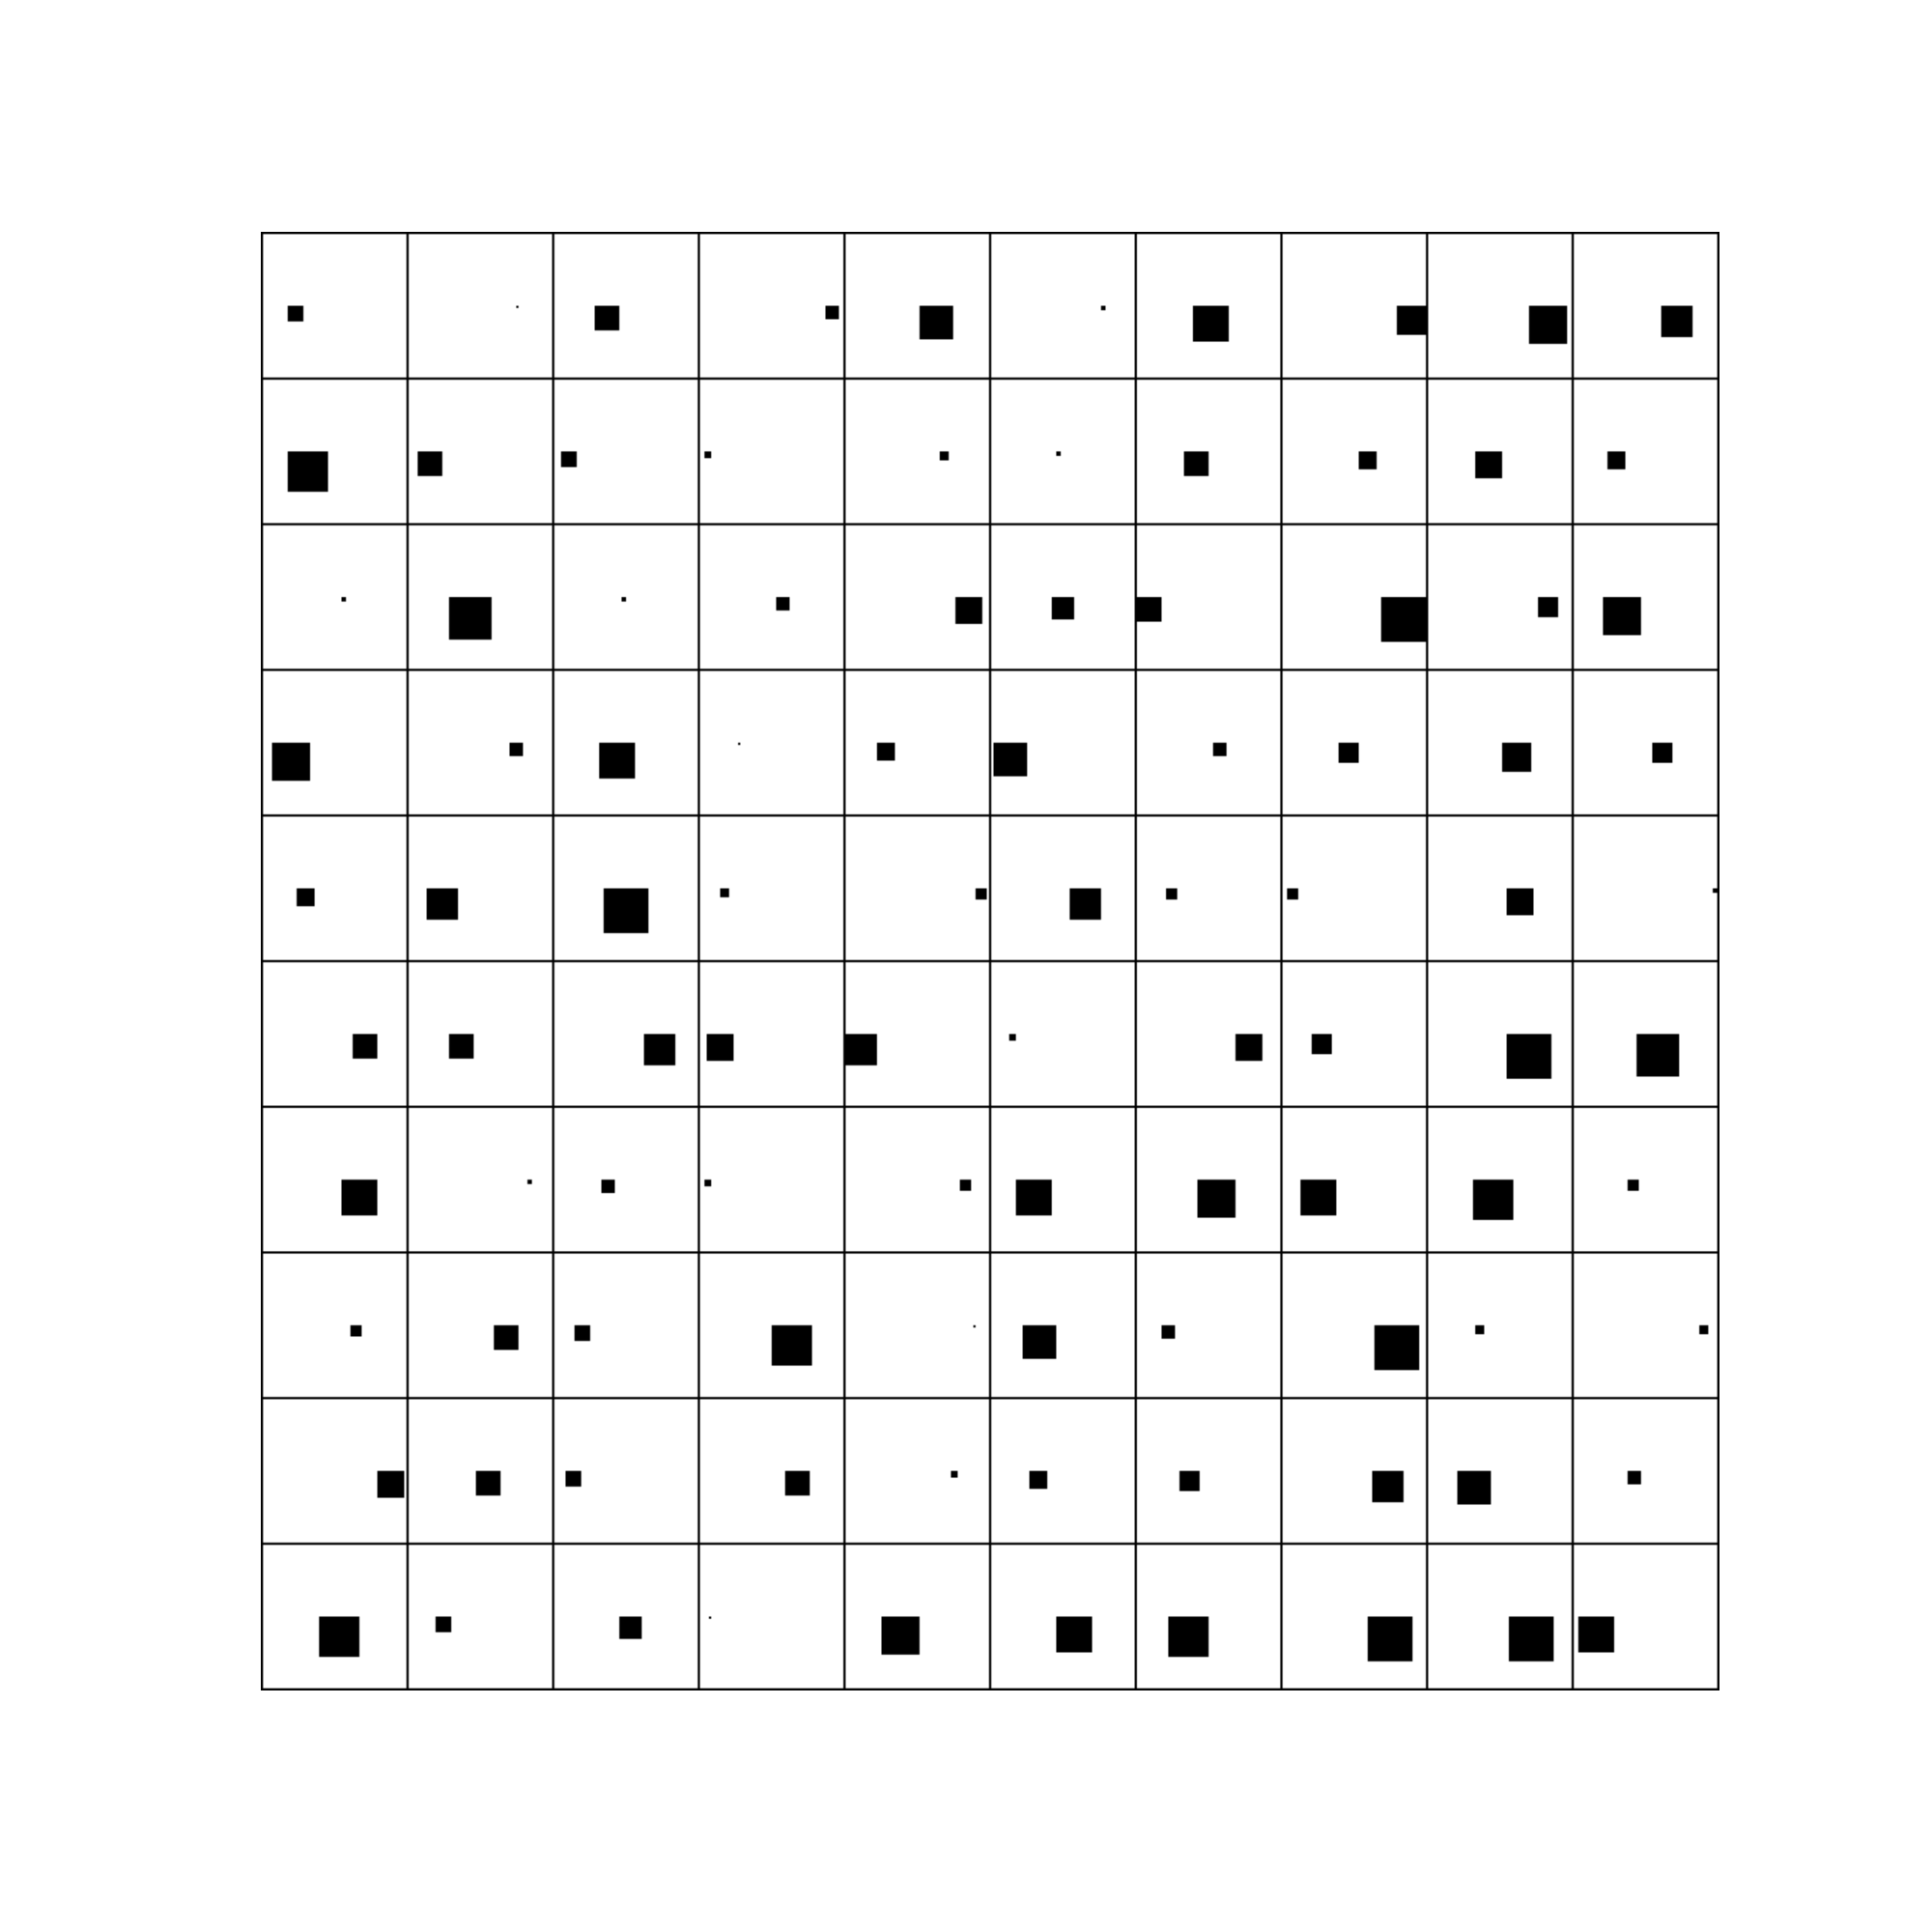
\includegraphics[width=0.6\textwidth]{shapes-train-data-samples.png}
    \caption{Sample images from our 2D squares dataset.}
    \label{fig:shape-samples}
\end{figure}

\subsubsection{Arithmetic Expression Fitting Task}
We follow \citet{kusner_grammar_2017} and optimise in the space of single-variable
arithmetic expressions generated by the formal grammar
\begin{align*}
    &\texttt{S $\rightarrow$ S '+' T | S '*' T | S '/' T | T}\\
    &\texttt{T $\rightarrow$ '(' S ')' | 'sin(' S ')' | 'exp(' S ')'}\\
    &\texttt{T $\rightarrow$ 'v' | '1' | '2' | '3'}\ ,
\end{align*}
where \texttt{S} and \texttt{T} denote non-terminals and the symbol \texttt{|}
separates the possible production rules generated from each non-terminal.
Every string in the dataset was generated by applying at most 15 production rules,
yielding arithmetic expressions such as \texttt{sin(2)}, \texttt{v/(3+1)} and \texttt{v/2 * exp(v)/sin(2*v)},
which are all considered to be functions of the variable \texttt{v}.
Following \citet{kusner_grammar_2017}, the objective is to find an expression
with minimal mean squared error to the target expression $\x^* = \texttt{1/3 * v * sin(v*v)}$,
computed over 1000 values of \texttt{v} evenly-spaced between $-10$ and $+10$.
In contrast to the original dataset of size 100,000 used by \citet{kusner_grammar_2017},
which \emph{includes the target expression} and many other well-performing inputs
(thus making the optimisation problem easy in theory), we make the task more challenging
by discarding the 50\% of points with the highest scores, resulting in a dataset of
size 50,000 with objective function value distribution shown in \cref{fig:weighting_equation}.
\paragraph{Data} 50,000 univariate arithmetic expressions generated by the formal grammar from \citet{kusner_grammar_2017}.
\paragraph{Model} A grammar \gls{vae} \citet{kusner_grammar_2017},
chosen because of its ability to produce only valid grammatical expressions.
Our implementation of the grammar \gls{vae} is based on the code from 
\citep{kusner_grammar_2017} provided at \url{https://github.com/mkusner/grammarVAE},
which we modified to use Tensorflow 2 \citep{abadi2016tensorflow} and python 3.
\paragraph{Latent optimiser} Bayesian optimisation with the expected improvement acquisition function \citep{jones1998efficient}
and a \glsfirst{sgp} model with 500 inducing points \citep{titsias2009variational},
following \citet{kusner_grammar_2017}.
We re-implemented the outdated and inefficient \texttt{Theano}-based Bayesian optimisation
implementation\footnote{see \url{https://github.com/mkusner/grammarVAE}}
of \citet{kusner_grammar_2017} (which was also used by \citep{jin_junction_2019})
using the popular and modern \texttt{Tensorflow 2.0}-based \texttt{GPflow} Gaussian process library
\citep{de2017gpflow} to benefit from GPU acceleration.
For computational efficiency, we fit the \gls{sgp} only on a subset of the data, consisting of the 2000 points
with the highest objective function values,
and 8000 randomly chosen points.
This also has the effect of ensuring that the \gls{sgp} properly fits the high-performing regions of the data.
Disregarding computational efficiency, we nonetheless found that fitting on this data subset remarkably improved performance
of the optimisation, even using the baseline model (without weighted retraining).

\begin{figure}[ht]
    \centering
    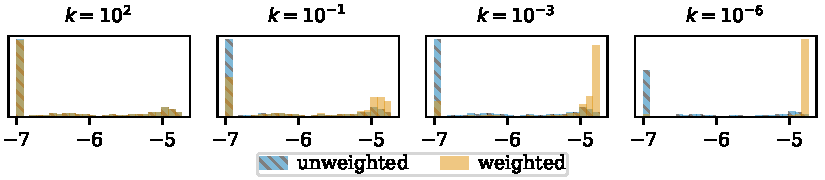
\includegraphics{histograms/train-data-hist-expr.pdf}
    \caption[Rank weighting on the arithmetic expression dataset.]{
    Illustration of rank weighting (\cref{eq:weighting_function})
    on the arithmetic expression dataset (defined in \cref{sec:lso:experiments}).
    }
    \label{fig:weighting_equation}
\end{figure}

\subsubsection{Chemical Design Task}
We follow \citet{gomez2018} and optimise the drug properties of molecules.
In particular, we consider the standardized task originally proposed in \citet{gomez2018}
of synthesizing a molecule with maximal penalized \emph{water-octanol partition coefficient} (logP),
starting from the molecules in the ZINC250k molecule dataset \citep{irwin_zinc_2012}.
The precise scoring function for a chemical $\x$ is defined as:
\begin{equation*}
\text{score}(\x) = \max\left(\widehat{\log{P}(\x)} -\widehat{\text{SA}(\x)} - \widehat{\text{cycle}(\x)}, \ -4\right)
\end{equation*}
where $\log{P}$, SA, and cycle are property functions,
and the $\ \widehat{}\ $ operation indicates standard normalization of the raw function output using the ZINC training set data
(i.e.\@ subtracting the mean of the training set, and dividing by the standard deviation).
This is identical to the scoring function from references \citep{kusner_grammar_2017,dai_syntax-directed_2018,jin_junction_2019,zhou_optimization_2019,you_graph_2018},
except that we bound the score below by $-4$ to prevent points with highly-negative scores from substantially impacting the optimisation procedure.
Functionally, because this is a maximisation task, this makes little difference to the scoring of the outcomes,
but does substantially help the optimisation.
This task has been studied in a long series of papers performing optimisation in chemical space,
allowing the effect of weighted retraining to be quantitatively compared to other optimisation approaches
\citep{kusner_grammar_2017,dai_syntax-directed_2018,jin_junction_2019,zhou_optimization_2019,you_graph_2018}.
\paragraph{Data} The ZINC250k molecule dataset \citep{irwin_zinc_2012}, using the same train/test split as \citep{jin_junction_2019}.
\paragraph{Model} A junction tree \gls{vae} \citep{jin_junction_2019},
chosen because it is a state-of-the-art \gls{vae} for producing valid chemical structures.
For direct comparability to previous results,
we use the pre-trained model provided in the code repository of \citep{jin_junction_2019} as the unweighted model,
and create weighted models by fine-tuning the pre-trained model for 1 epoch over the full weighted dataset.
\paragraph{Latent optimiser} Same as for the arithmetic expression task.


\subsection{Effect of Weighted Training}
\label{subsec:expt-weighting}
In this section, we seek to validate some of the conjectures made in \cref{sec:lso:limitations,sec:lso:main},
namely that 1) the latent space of a \gls{dgm} trained on uniformly weighted data contains many poor-performing points, and 2) that weighted training fixes this by introducing more high-performing points into the latent space.
To test this, we train a \gls{vae} for each task using rank weighting with a variety of $k$ values (noting that $k=\infty$ corresponds to uniform weighting), initializing the weights using a pre-trained \gls{vae} to ensure that the different runs are comparable.
We evaluate $f$ on samples from the \gls{dgm}'s prior for each task, and plot the resulting distributions in \cref{fig:prior-samples} with the label \emph{before retraining}.
Although the distribution of scores for $k=\infty$ does not exactly match the training distribution
for any example, it tends to have a similar range, showing that much of the latent space is dedicated to modelling low-scoring points.
Weighted training robustly causes the distribution to skew towards higher values at the expense of lower values, which is exactly the intended effect.
The upshot is that the result on all 3 tasks broadly supports our conjectures.

\begin{figure}[ht]
    \centering
    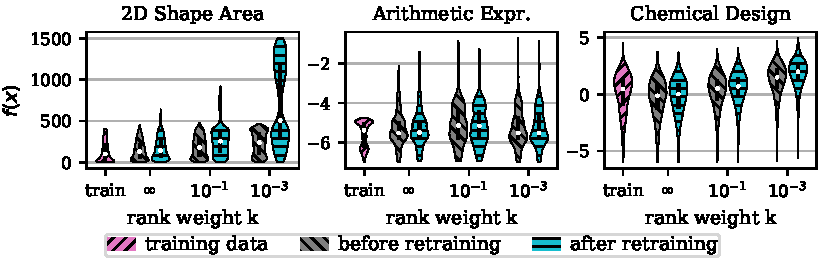
\includegraphics{violin.pdf}
    \caption[Prior samples from the \gls{dgm}'s prior for all tasks.]{
    Objective value distribution for the training set and samples from the \gls{dgm}'s prior
    for all three tasks for different $k$ values,
    before and after weighted retraining (see \cref{subsec:expt-wr}).
    }
    \label{fig:prior-samples}
\end{figure}


\subsection{Effect of Weighted Retraining Parameters on optimisation}
\label{subsec:expt-wr}
When using rank-weighting from \cref{eq:weighting_function} with parameter $k$ and picking a fixed period for model retraining $r$,
\gls{lmo} with weighted retraining can be completely characterized by $k$ and $r$.
The baseline of uniform weighting and no retraining is represented by $k=r=\infty$,
with decreasing values of $k$ and $r$ representing more skewed weighting and more frequent retraining, respectively.
For each task, we choose a value $r_\text{low}$ based on our computational retraining budget,
then perform \gls{lmo} for each value of 
$k\in\{k_{\text{low}}, \infty \}$ and $r\in\{r_{\text{low}}, \infty \}$.
For computational efficiency retraining is done via fine-tuning.

The results are shown in \cref{fig:wr-params}.
Firstly, comparing the case of $k=\infty,r=\infty$ with $k=\infty,r=r_{\text{low}}$ and $k=k_{\text{low}},r=\infty$
suggests that both weighting and retraining help individually, as hypothesized in \cref{sec:lso:main}.
Secondly, in all cases, weighted retraining with $k=k_{\text{low}},r=r_{\text{low}}$ performs better than all other methods, suggesting that they have a synergistic effect when combined.
Note that the performance often increases suddenly after retraining,
suggesting that the retraining does indeed incorporate new information into the latent space, as conjectured.
Lastly, the objective function values of prior samples from the models after weighted retraining
with $r=r_{\text{low}}$ is shown in \cref{fig:prior-samples} in blue.
In all cases, the distribution becomes more skewed towards positive values, with the difference being more pronounced for lower $k$ values.
This suggests that weighted retraining is able to significantly modify the latent space, even past the initial retraining.

\begin{figure}[th]
    \centering
    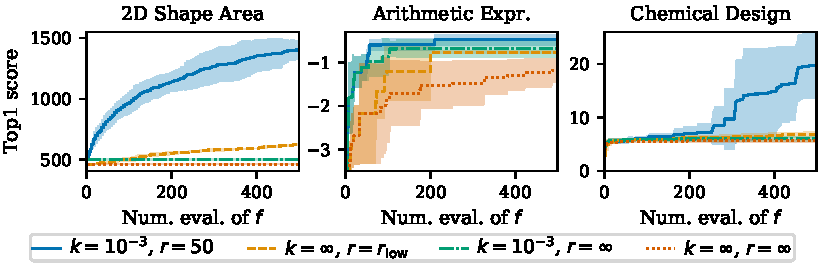
\includegraphics{optimization-top1.pdf}
    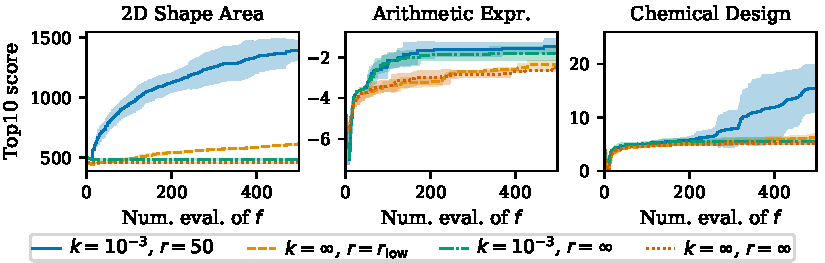
\includegraphics{optimization-top10.pdf}
    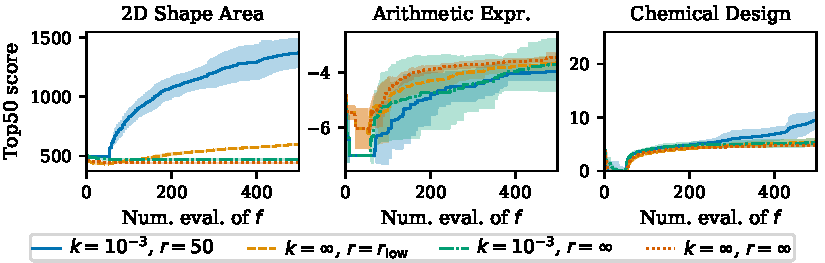
\includegraphics{optimization-top50.pdf}
    \caption[Top$1$, $10$, and $50$ optimisation performance of weighted retraining for all tasks.]{
        Top$1$, $10$, and $50$ optimisation performance of weighted retraining for all tasks,
        for different $k$ values (i.e.\@ $k \in \{10^{-3}, \infty\}$)
        and retraining frequencies (i.e.\@ $r_\text{low} = 5$ for the 2D shape area task,
        and $r_\text{low} = 50$ for the other two tasks). Shaded area corresponds to standard deviation.
    }
    \label{fig:wr-params}
\end{figure}


\subsection{Comparison with Other Methods}
\label{subsec:expt-baselines}
Finally, we compare our proposed method of \gls{lmo} (with weighted retraining) with other methods on the same tasks.
The first class of methods are based on the cross-entropy method as discussed in \cref{sec:lso:related-work},
namely design by adaptive sampling (DbAS) \citep{Brookes_Listgarten_2020},
the cross-entropy method with probability of improvement (CEM-PI) \citep{rubinstein_cross-entropy_1999},
the feedback VAE (FBVAE) \citep{gupta_feedback_2019} and reward-weighted regression (RWR)
\citep{peters2007reinforcement}.
These methods are noteworthy because they can be viewed as a particular case of weighted retraining,
where the weights are binary (except for DbAS)
and the latent optimiser simply consists of sampling from the \gls{dgm}'s prior.
The hyperparameters of these methods are the sequence of quantiles, and the retraining frequency.
We optimise these hyperparameters using a grid search.

\Cref{fig:baselines} shows the performance of these methods on the best hyperparameter setting found, as a function of the number of samples drawn (with a budget of 5,000 samples in total).
We plot the average and standard deviation across 3 random seeds, as we found the variances to be relatively low.
We observe that all other forms of weighted retraining perform significantly worse than our own,
failing to achieve the performance of our approach, even with an evaluation budget that is an order of magnitude larger than ours (i.e.\@ 5,000 vs 500).
We attribute this both to their binary weighting scheme and their lack of a sample-efficient latent optimiser.

\begin{figure}[htb]
    \centering
    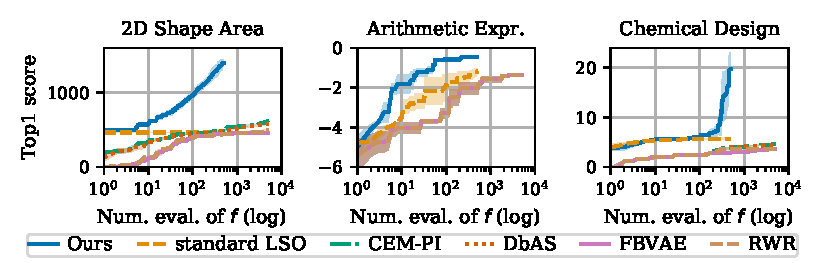
\includegraphics[width=\textwidth]{baselines.pdf}
    \caption[Comparison of weighted retraining, LSO, CEM-PI, DbAS, FBVAE and RWR.]{
        Comparison of weighted retraining, LSO, CEM-PI, DbAS, FBVAE and RWR.
        Our weighted retraining approach significantly outperforms all baselines, achieving both better sample-efficiency and final performance.
    }
    \label{fig:baselines}
\end{figure}

Secondly, we compare against other methods in the literature that have attempted the same chemical design task.
To our knowledge, the best previously reported score obtained using a machine learning method is 11.84 and was obtained with $\approx5000$ samples \citep{zhou_optimization_2019}.
By contrast, our best score is \bestchemscore{} and was achieved with only 500 samples.
Expanding the scope to include more domain-specific optimisation methods,
we acknowledge that ChemBO achieved an impressive score of 18.39 in only 100 samples \citep{korovina2020chembo},
which is better than our method's performance with only 100 samples.
\Cref{tab:chem-results} gives a more detailed comparison with other work.
\Cref{fig:best-molecule-pix} illustrates some of the best molecules found with weighted retraining.
Note that all the high-scoring molecules are extremely large.
It has been reported previously that larger molecules achieve higher scores,
thereby diminishing the impressiveness of this particular design task for \gls{rl} algorithms \citep{zhou_optimization_2019}.
However, the fact that these molecules were found with a generative model strongly highlights
the ability of weighted retraining to find solutions outside of the original training distribution.

\begin{table}[h]
  \centering
  \begin{tabular}{lllll}
    \toprule
    \textbf{Model}     & \textbf{1st}     & \textbf{2nd} & \textbf{3rd} & \textbf{no.\@ queries } \\
    \midrule
    JT-VAE \citep{jin_junction_2019} & 5.30  & 4.93 & 4.49 & $2500^\dagger$     \\
    GCPN \citep{you_graph_2018}     & 7.98 & 7.85 & 7.80 & $\approx10^{6\ddagger}$     \\
    MolDQN \citep{zhou_optimization_2019} & 11.84 & 11.84 & 11.82 & $\geq5000^*$  \\
    ChemBO \citep{korovina2020chembo} & 18.39 & - & - & \textbf{100}$^{**}$ \\
    \midrule
    \textbf{JT-VAE} (our Bayesian optimisation) & 5.65 & 5.63 & 5.43 & 500 \\
    \textbf{JT-VAE} ($k=10^{-3}$, no retraining) & 5.95 & 5.75 & 5.72 & 500 \\
    \textbf{JT-VAE} ($k=10^{-3}$, retraining) & 21.20 & 15.34 & 15.34 & 500 \\
    \textbf{JT-VAE} ($k=10^{-3}$, retraining, \emph{best result}) & \textbf{27.84} & \textbf{27.59} & \textbf{27.21} & \textbf{500} \\
    \bottomrule
  \end{tabular}
  \caption[Comparison of top 3 scores on chemical design task.]{
    Comparison of top 3 scores on chemical design task.
  Baseline results are copied from \citep{zhou_optimization_2019}.
  All our results state the \emph{median} of 5 runs unless otherwise stated (judged by best result),
  each run being 500 epochs.
  $^\dagger$These were the top results across 10 seeds, with 250 queries performed per seed.
  $^\ddagger$Obtained through email correspondence with the authors.
  $^*$The experimental section states that the model was trained for 5000 episodes,
  so at least 5000 samples were needed.
  It is unclear if any batching was used, which would make the number of samples greater.
  $^{**}$From table 3 of \citet{korovina2020chembo}.
  }
  \label{tab:chem-results}
\end{table}

\begin{figure}[ht]
    \centering
    \begin{tikzpicture}
        \draw (0, 0) node[inner sep=0] {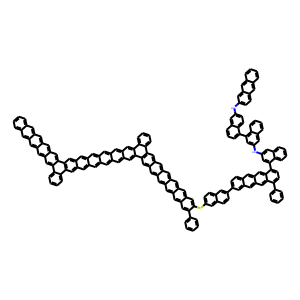
\includegraphics[width=0.3\linewidth]{{mol_pictures/mol_27.84}.png}};
        \draw (0, 1) node {27.84};
    \end{tikzpicture}
    \begin{tikzpicture}
        \draw (0, 0) node[inner sep=0] {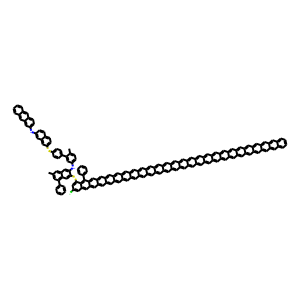
\includegraphics[width=0.3\linewidth]{{mol_pictures/mol_27.59}.png}};
        \draw (1, 1) node {27.59};
    \end{tikzpicture}
    \begin{tikzpicture}
        \draw (0, 0) node[inner sep=0] {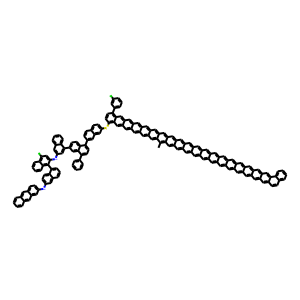
\includegraphics[width=0.3\linewidth]{{mol_pictures/mol_27.21}.png}};
        \draw (1, 1) node {27.21};
    \end{tikzpicture}
    \begin{tikzpicture}
        \draw (0, 0) node[inner sep=0] {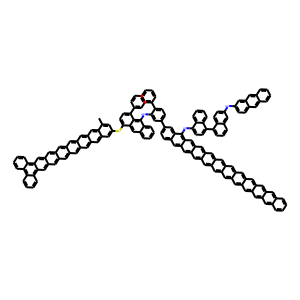
\includegraphics[width=0.3\linewidth]{{mol_pictures/mol_25.90}.png}};
        \draw (1, 1) node {25.90};
    \end{tikzpicture}
    \begin{tikzpicture}
        \draw (0, 0) node[inner sep=0] {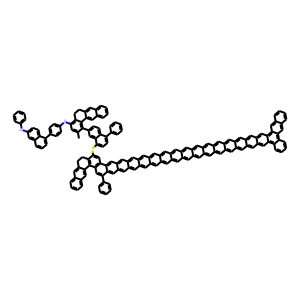
\includegraphics[width=0.3\linewidth]{{mol_pictures/mol_25.37}.png}};
        \draw (1, 1) node {25.37};
    \end{tikzpicture}

    \caption[Molecules found by LSO with logP scores.]{Some of the best molecules for the logP maximisation task found using weighted retraining. Numbers indicate the logP score of each molecule.}
    \label{fig:best-molecule-pix}
\end{figure}
